% =====================================================================
%  Section 2.1  —  LLM Foundations : all diagrams in TikZ
% ---------------------------------------------------------------------
%  HOW TO USE
%  • Compile on Overleaf / Prism (pdfLaTeX). Because this uses the
%    `standalone' class with the [tikz] option, EACH tikzpicture becomes
%    its OWN cropped page in the output PDF — one diagram per page.
%  • To get images for Prezi: open the PDF, export/save each page as
%    PNG (or SVG). In Prezi: Insert > Image.
%  • To reuse a single diagram inside your thesis: copy ONE
%    \begin{tikzpicture}...\end{tikzpicture} block into a figure
%    environment (make sure the preamble packages/colours below exist).
%
%  Colour key (consistent everywhere):
%    cmpute (blue) = compute / Prefill      memr (red) = memory / Decode
% =====================================================================
\documentclass[tikz,border=12pt]{standalone}
\usepackage{amsmath}
\usepackage{amssymb}   % \checkmark
\usepackage{booktabs}
\usepackage{array}
\usetikzlibrary{positioning,calc,arrows.meta,shapes.geometric,backgrounds,fit,
                decorations.pathreplacing}

% ---------- palette ----------
\definecolor{cmpute}{HTML}{1F6FB2}
\definecolor{memr}{HTML}{C0392B}
\definecolor{dark}{HTML}{222B33}
\definecolor{gold}{HTML}{E08E0B}
\definecolor{grn}{HTML}{2E8B57}
\definecolor{lblue}{HTML}{D6E6F4}
\definecolor{lred}{HTML}{F6DEDB}
\definecolor{lgrey}{HTML}{ECF0F3}
\definecolor{mgrey}{HTML}{6B737B}

% ---------- shared styles ----------
\tikzset{
  every node/.append style={font=\sffamily},
  box/.style={rounded corners=3pt, align=center, inner sep=7pt,
              font=\sffamily\bfseries, minimum height=1cm},
  prompt/.style={box, fill=dark, text=white, minimum width=4.4cm, minimum height=1.1cm},
  llm/.style={box, fill=cmpute, text=white, minimum width=1.8cm, minimum height=1.1cm},
  proc/.style={box, fill=cmpute, text=white, minimum width=2cm},
  procd/.style={box, fill=dark, text=white},
  data/.style={box, fill=lgrey, draw=mgrey, text=dark, font=\sffamily},
  tok/.style={rounded corners=2pt, fill=cmpute, text=white,
              minimum size=0.72cm, inner sep=1pt, font=\sffamily\bfseries},
  arr/.style={-{Stealth[length=3mm]}, line width=1pt, draw=mgrey},
  arrd/.style={-{Stealth[length=3mm]}, line width=1.1pt, draw=dark},
  arrr/.style={-{Stealth[length=3mm]}, line width=1.1pt, draw=memr},
  cap/.style={box, font=\sffamily, align=center, inner sep=9pt},
  capb/.style={cap, fill=lblue, draw=cmpute, line width=1pt, text=dark},
  capr/.style={cap, fill=lred,  draw=memr,   line width=1pt, text=dark},
  capg/.style={cap, fill=lgrey, draw=mgrey,  line width=1pt, text=dark},
  ttl/.style={font=\sffamily\bfseries\large, text=dark},
}

\begin{document}

% =====================================================================
% P1 — What is an LLM? (next-token predictor)
% =====================================================================
\begin{tikzpicture}
  \node[ttl] at (5.4,2.4) {P1 \quad What is an LLM?  \;— a next-token predictor};
  \node[prompt] (q) at (0,0) {"The cat sat on the \_\_\_"};
  \node[llm]    (m) at (5.4,0) {LLM};
  \draw[arr] (q) -- (m);
  % probability bars
  \def\bx{7.5}
  \foreach \i/\w/\lbl/\pct/\col in
     {0/3.0/mat/62\%/memr, 1/0.9/floor/18\%/mgrey, 2/0.45/roof/9\%/mgrey,
      3/0.27/box/5\%/mgrey, 4/0.12/{...}/2\%/mgrey}{
     \node[anchor=east, font=\sffamily\bfseries] at (\bx-0.15,-\i*0.7) {\lbl};
     \fill[\col] (\bx,-\i*0.7-0.2) rectangle (\bx+\w,-\i*0.7+0.2);
     \node[anchor=west, font=\sffamily\small, text=mgrey] at (\bx+\w+0.12,-\i*0.7) {\pct};
  }
  \draw[arr] (m) -- (\bx-0.2,0);
  \node[capr, text width=12cm] at (5.4,-3.2)
    {It outputs a probability for \emph{every} possible next word
     $\rightarrow$ pick the top one $\rightarrow$ append $\rightarrow$ repeat.
     \\ Generating text = doing this tiny prediction over and over.};
\end{tikzpicture}

% =====================================================================
% P2 — Text -> Tokens -> Vectors
% =====================================================================
\begin{tikzpicture}[node distance=0.7cm]
  \node[ttl] at (7,2.0) {P2 \quad Text $\rightarrow$ Tokens $\rightarrow$ Vectors};
  \node[prompt, minimum width=2.6cm] (w) {"unbelievable"};
  \node[proc, right=of w]  (tk)  {TOKENIZER};
  \node[data, right=of tk] (tok) {["un","believ","able"]};
  \node[proc, right=of tok] (emb) {EMBEDDING};
  \node[data, right=of emb] (vec) {$[\,0.2,\,-1.3,\,0.9,\,\ldots\,]$};
  \draw[arr] (w)--(tk);  \draw[arr] (tk)--(tok);
  \draw[arr] (tok)--(emb); \draw[arr] (emb)--(vec);
  \node[font=\sffamily\small, text=mgrey] at ($(w)+(0,-0.8)$) {text};
  \node[font=\sffamily\small, text=mgrey] at ($(tok)+(0,-0.8)$) {word pieces};
  \node[font=\sffamily\small, text=mgrey] at ($(vec)+(0,-0.8)$) {a vector of numbers};
  \node[capb, text width=13cm] at (7,-2.2)
    {\textbf{Meaning becomes geometry:}\quad
     king $-$ man $+$ woman $\approx$ queen \quad
     (vectors that are \emph{close} = meanings that are \emph{similar}).};
\end{tikzpicture}

% =====================================================================
% P3 — Parameters = stored knowledge
% =====================================================================
\begin{tikzpicture}
  \node[ttl] at (6,2.6) {P3 \quad Parameters = stored knowledge};
  \node[llm, minimum width=4.4cm, minimum height=1.5cm,
        font=\sffamily\bfseries\Large] (mm) at (0,0) {SmolLM2-135M};
  \node[font=\sffamily\bfseries, text=dark] at (0,-1.2) {135{,}000{,}000 parameters};
  \draw[arrd] (mm.east) -- ++(1.1,0);
  \node[capg, text width=5cm, anchor=west] at (3.6,0)
    {Every weight must be \textbf{stored} in memory and \textbf{read} for each token generated.};
  \node[capr, text width=12.5cm] at (6,-2.7)
    {\textbf{Seed of the whole story:} reading all these numbers, for every single token,
     is the bottleneck we meet soon.\\
     135M params $\rightarrow$ $\sim$141\,MB at INT4 $\rightarrow$ must fit in the board's DDR3.};
\end{tikzpicture}

% =====================================================================
% P4 — Train once, run forever
% =====================================================================
\begin{tikzpicture}
  \node[ttl] at (6,3.0) {P4 \quad Train once, run forever};
  \node[capb, text width=5cm, minimum height=2.6cm, anchor=north] (tr) at (0,2.2)
    {\textcolor{cmpute}{\bfseries\large TRAINING}\\[4pt]
     \begin{minipage}{4.4cm}\raggedright\sffamily
     $\bullet$ done ONCE $\cdot$ takes weeks\\
     $\bullet$ needs many GPUs\\
     $\bullet$ learns the weights\\
     $\bullet$ then weights are FROZEN
     \end{minipage}};
  \node[capr, text width=5cm, minimum height=2.6cm, anchor=north] (inf) at (8,2.2)
    {\textcolor{memr}{\bfseries\large INFERENCE}\\[4pt]
     \begin{minipage}{4.4cm}\raggedright\sffamily
     $\bullet$ done EVERY request\\
     $\bullet$ weights are fixed\\
     $\bullet$ prompt in $\rightarrow$ output out\\
     $\bullet$ \textbf{our project lives here}
     \end{minipage}};
  \draw[arrd] (tr.east) -- node[above,font=\sffamily\small\itshape,text=mgrey]{weights} (inf.west);
  \node[capg, text width=12.5cm] at (4,-1.3)
    {Training learns the numbers. \; Inference uses them. \; \textbf{We only do inference.}\\
     And inference itself splits into TWO phases\,$\rightarrow$};
\end{tikzpicture}

% =====================================================================
% P5 — The Transformer (stack of decoder layers)
% =====================================================================
\begin{tikzpicture}
  \node[ttl] at (3.4,3.2) {P5 \quad The Transformer};
  \foreach \i/\lbl/\col in
     {0/{DECODER LAYER}/cmpute, 1/{DECODER LAYER}/cmpute,
      2/{DECODER LAYER}/cmpute, 3/{DECODER LAYER ($\times$ 30)}/dark}{
     \node[box, fill=\col, text=white, minimum width=5cm] (L\i) at (0,\i*0.85) {\lbl};
  }
  \node[font=\sffamily\bfseries, text=dark, anchor=east] at (-2.7,0) {text in};
  \draw[arr] (-2.6,0) -- (L0.west);
  \draw[arr] (L3.north) -- ++(0,0.7)
        node[above,font=\sffamily\bfseries,text=dark]{next token out};
  \node[capg, text width=3.4cm, minimum height=2.6cm, anchor=west] (lay) at (3.2,1.3)
    {each layer =\\[6pt]\textbf{Attention}\\$+$\\\textbf{Feed-Forward (FFN)}};
  \draw[arr] (lay.west) -- (L1.east);
  \node[font=\sffamily\itshape, text=mgrey] at (1.8,-1.4)
    {SmolLM2-135M = 30 layers, hidden size 2048};
\end{tikzpicture}

% =====================================================================
% FRAME 1 — Two phases (HERO)
% =====================================================================
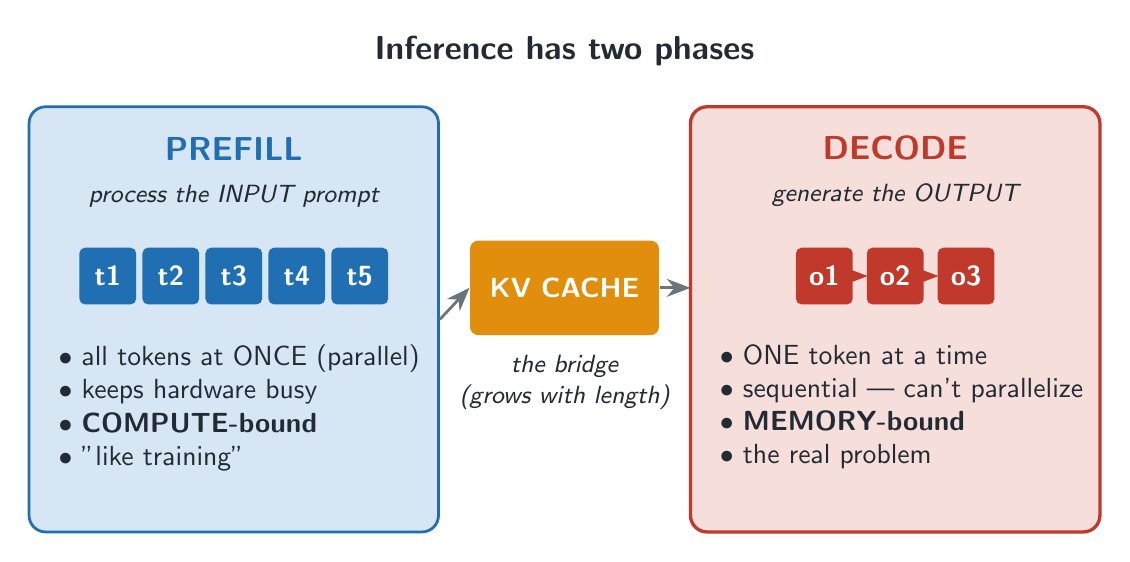
\begin{tikzpicture}
  \node[ttl] at (4.2,3.4) {Inference has two phases};
  % --- Prefill panel ---
  \node[draw=cmpute,line width=1pt,fill=lblue,rounded corners=6pt,
        minimum width=5.2cm,minimum height=5.4cm] (pf) at (0,0){};
  \node[font=\sffamily\bfseries\large,text=cmpute] at ([yshift=-0.55cm]pf.north){PREFILL};
  \node[font=\sffamily\itshape\small,text=dark] at ([yshift=-1.15cm]pf.north){process the INPUT prompt};
  \foreach \i/\x in {1/-1.6,2/-0.8,3/0,4/0.8,5/1.6}{
     \node[tok, fill=cmpute] at (\x,0.55){t\i};}
  \node[anchor=north west,align=left,text=dark,font=\sffamily] at (-2.35,-0.2)
    {$\bullet$ all tokens at ONCE (parallel)\\
     $\bullet$ keeps hardware busy\\
     $\bullet$ \textbf{COMPUTE-bound}\\
     $\bullet$ "like training"};
  % --- KV bridge ---
  \node[box, fill=gold, text=white, minimum width=2.4cm, minimum height=1.2cm] (kv) at (4.2,0.4){KV CACHE};
  \node[font=\sffamily\itshape\small,text=dark,align=center] at (4.2,-0.8){the bridge\\(grows with length)};
  \draw[arr] (pf.east) -- (kv.west);
  \draw[arr] (kv.east) -- (5.8,0.4);
  % --- Decode panel ---
  \node[draw=memr,line width=1.2pt,fill=lred,rounded corners=6pt,
        minimum width=5.2cm,minimum height=5.4cm] (dc) at (8.4,0){};
  \node[font=\sffamily\bfseries\large,text=memr] at ([yshift=-0.55cm]dc.north){DECODE};
  \node[font=\sffamily\itshape\small,text=dark] at ([yshift=-1.15cm]dc.north){generate the OUTPUT};
  \foreach \i/\x in {1/7.5,2/8.4,3/9.3}{
     \node[tok, fill=memr] at (\x,0.55){o\i};}
  \draw[arrr,line width=0.9pt] (7.85,0.55)--(8.05,0.55);
  \draw[arrr,line width=0.9pt] (8.75,0.55)--(8.95,0.55);
  \node[anchor=north west,align=left,text=dark,font=\sffamily] at (6.05,-0.2)
    {$\bullet$ ONE token at a time\\
     $\bullet$ sequential — can't parallelize\\
     $\bullet$ \textbf{MEMORY-bound}\\
     $\bullet$ the real problem};
\end{tikzpicture}

% =====================================================================
% FRAME 2 — Autoregressive loop
% =====================================================================
\begin{tikzpicture}
  \node[ttl] at (5,2.2) {The autoregressive loop};
  \node[font=\sffamily\bfseries,text=dark] at (5,1.5)
    {auto = self \quad$\cdot$\quad regressive = depends on previous outputs};
  \node[prompt,minimum width=1.5cm] (a) at (0,0){"The"};
  \node[llm]    (b) at (2.3,0){MODEL};
  \node[prompt,minimum width=1.5cm] (c) at (4.6,0){"cat"};
  \node[llm]    (d) at (6.9,0){MODEL};
  \node[prompt,minimum width=1.5cm] (e) at (9.2,0){"sat"};
  \node[font=\sffamily\bfseries,text=mgrey] at (10.6,0){$\ldots$};
  \foreach \s/\t in {a/b,b/c,c/d,d/e}{\draw[arr] (\s)--(\t);}
  % feedback loop
  \draw[arrr] (c.south) |- (-0.9,-1.3) -| (a.south);
  \node[font=\sffamily\bfseries,text=memr] at (1.9,-1.55){feed the output back in};
  \node[capr, text width=11cm] at (5,-2.7)
    {One token at a time $\rightarrow$ you can't compute token \#2 before token \#1 exists
     $\rightarrow$ no parallelism $\rightarrow$ \textbf{DECODE is memory-bound.}};
\end{tikzpicture}

% =====================================================================
% FRAME 3 — Inside a decoder layer
% =====================================================================
\begin{tikzpicture}[node distance=0.55cm]
  \node[ttl] at (6,2.6) {Inside a decoder layer};
  \node[procd, minimum width=1.6cm] (t) at (0,1){text};
  \node[proc, right=of t] (em){EMBEDDING};
  \node[procd, right=of em, minimum width=3.4cm] (dl){DECODER LAYER $\times$ N};
  \node[proc, right=of dl, minimum width=2.4cm] (lh){LM HEAD $\rightarrow$ next token};
  \draw[arr](t)--(em); \draw[arr](em)--(dl); \draw[arr](dl)--(lh);
  \draw[arr] (dl.south) -- ++(0,-0.55);
  \node[capb, text width=3.8cm, minimum height=2.4cm, anchor=north] (att) at (3,-0.6)
    {\textcolor{cmpute}{\bfseries ATTENTION}\\[4pt]
     "gather context from other words"\\[4pt]
     \emph{latency-sensitive}\\(many quick comparisons)};
  \node[capr, text width=3.8cm, minimum height=2.4cm, anchor=north] (ffn) at (8,-0.6)
    {\textcolor{memr}{\bfseries FFN}\\[4pt]
     "think about it individually"\\[4pt]
     \emph{weight-intensive}\\(lots of stored data)};
\end{tikzpicture}

% =====================================================================
% FRAME 4 — Attention = Q, K, V
% =====================================================================
\begin{tikzpicture}
  \node[ttl] at (6,3.2) {Attention = Q, K, V};
  \foreach \i/\k/\d/\col in
     {0/Q/{what am I looking for?}/cmpute,
      1/K/{what do I offer?}/gold,
      2/V/{my actual content}/grn}{
     \node[box, fill=\col, text=white, minimum width=0.9cm, minimum height=0.8cm,
           font=\sffamily\bfseries\large] (n\i) at (0,2-\i*0.95){\k};
     \node[anchor=west, font=\sffamily\bfseries, text=dark] at (0.7,2-\i*0.95){\d};
  }
  \node[procd, text width=6cm, minimum height=1.8cm] (flow) at (8.6,1.05)
    {score $=Q\!\cdot\!K^{\top}\ \rightarrow\ \div\sqrt{d_k}\ \rightarrow\ \mathrm{softmax}\ \rightarrow\ \times V$
     \\[4pt]\small\itshape\textcolor{lblue}{= a context-updated vector for the word}};
  \draw[arr] (3.3,1.05) -- (flow.west);
  \node[capg, text width=8.8cm, font=\sffamily\bfseries\Large] at (5,-0.7)
    {Attention $=\ \mathrm{softmax}\!\left(\dfrac{Q K^{\top}}{\sqrt{d_k}}\right) V$};
  \node[capb, text width=12cm] at (5,-2.8)
    {"The bank was closed because the river flooded."\\
     $\rightarrow$ "bank" attends to "river" $\rightarrow$ it means LAND, not money.};
\end{tikzpicture}

% =====================================================================
% FRAME 5 — The Memory Wall
% =====================================================================
\begin{tikzpicture}
  \node[ttl] at (3,4) {The Memory Wall — the "aha"};
  % axes
  \draw[arrd] (0,0) -- (0,3.6) node[above left,font=\sffamily\small\itshape,text=mgrey]{performance};
  \draw[arrd] (0,0) -- (6.4,0) node[below right,font=\sffamily\small\itshape,text=mgrey]{time};
  % compute (steep) and memory (shallow)
  \draw[-{Stealth[length=3mm]},line width=1.6pt,cmpute] (0.2,0.3) -- (5.8,3.3)
        node[above,font=\sffamily\bfseries,text=cmpute]{compute};
  \draw[-{Stealth[length=3mm]},line width=1.6pt,memr] (0.2,0.25) -- (5.8,1.3)
        node[right,font=\sffamily\bfseries,text=memr]{memory bandwidth};
  \node[align=center,font=\sffamily\bfseries,text=dark] at (4.4,2.0){THE GAP\\= memory wall};
  % table
  \node[anchor=north west] at (7.6,3.9){%
    \sffamily\footnotesize
    \renewcommand{\arraystretch}{1.3}
    \begin{tabular}{>{\bfseries}l l l c}
      \toprule
      Type & Speed & Density & Cost\\
      \midrule
      SRAM & very fast & low  & \$\$\$\\
      DRAM & slower    & high & \$\\
      HBM  & high BW   & high & \$\$\$\\
      \bottomrule
    \end{tabular}};
  \node[capr, text width=6cm, anchor=north west] at (7.6,1.0)
    {Decode lives in the memory-bound regime $\rightarrow$ it starves waiting for data.
     \\ \textbf{No GPU/TPU was designed just for decode.}};
\end{tikzpicture}

% =====================================================================
% FRAME 6 — Why a tiny model (funnel)
% =====================================================================
\begin{tikzpicture}
  \node[ttl] at (4,3.6) {Why a tiny model?};
  \node[capg, text width=8.4cm] at (4,2.7)
    {Many capable LLMs \;(7B, 13B, \ldots)\; — too big for the board};
  \node[box, fill=gold, text=white, minimum width=6.4cm] (c1) at (4,1.7)
    {constraint 1:\ 1\,GB DDR3 on ZC702};
  \node[box, fill=gold, text=white, minimum width=5.4cm] (c2) at (4,0.95)
    {constraint 2:\ 64-bit AXI bus @ 93.75\,MHz};
  \node[box, fill=memr, text=white, minimum width=4.4cm] (c3) at (4,0.2)
    {constraint 3:\ decoder-only + GQA runtime};
  \draw[arrd] (4,-0.35) -- (4,-0.85);
  \node[box, fill=grn, text=white, text width=5.6cm, minimum height=1.3cm] (sm) at (4,-1.6)
    {\large SmolLM2-135M\\[2pt]
     \normalsize 141\,MB @ INT4 $\cdot$ 30 layers $\cdot$ hidden 2048};
  \node[font=\sffamily\bfseries,text=dark] at (4,-2.7)
    {\checkmark\ fits \quad \checkmark\ all kernels verified \quad \checkmark\ compressible};
  \node[anchor=west,font=\sffamily\itshape\small,text=mgrey,align=left] at (8.0,-1.6)
    {Qwen2.5-0.5B = upgrade path\\(blocked: missing bias\\ tensors $\rightarrow$ future work)};
\end{tikzpicture}

% =====================================================================
% FRAME 7 — The spine (closing chain)
% =====================================================================
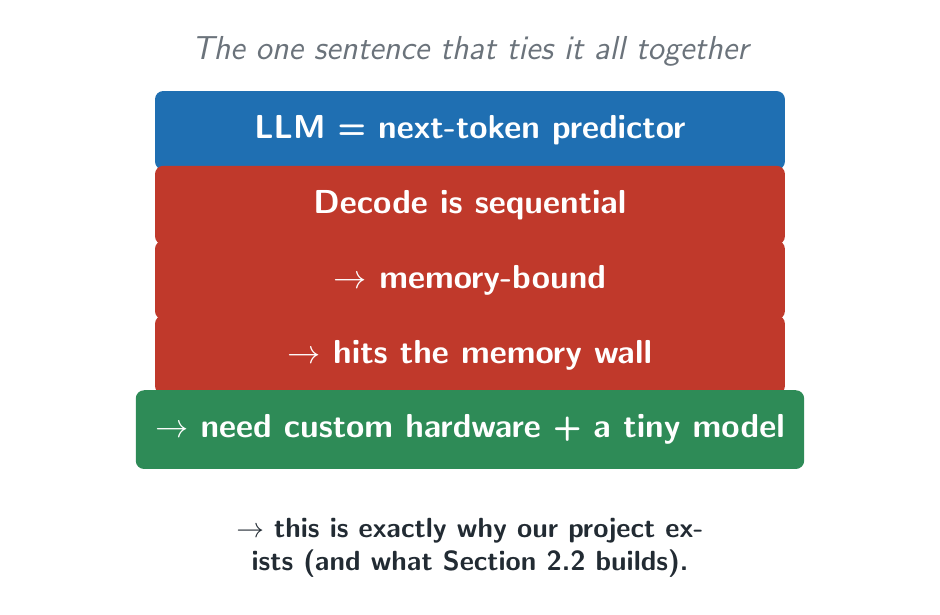
\begin{tikzpicture}
  \node[font=\sffamily\itshape\large,text=mgrey] at (0,3.0)
    {The one sentence that ties it all together};
  \foreach \i/\txt/\col in
     {0/{LLM = next-token predictor}/cmpute,
      1/{Decode is sequential}/memr,
      2/{$\rightarrow$ memory-bound}/memr,
      3/{$\rightarrow$ hits the memory wall}/memr,
      4/{$\rightarrow$ need custom hardware + a tiny model}/grn}{
     \node[box, fill=\col, text=white, minimum width=8cm,
           font=\sffamily\bfseries\large] at (0,2-\i*0.95){\txt};
  }
  \node[font=\sffamily\bfseries,text=dark,text width=11cm,align=center] at (0,-3.3)
    {$\rightarrow$ this is exactly why our project exists (and what Section 2.2 builds).};
\end{tikzpicture}

\end{document}
